%                                                                 aa.dem
% AA vers. 9.1, LaTeX class for Astronomy & Astrophysics
% demonstration file
%                                                       (c) EDP Sciences
%-----------------------------------------------------------------------
%
%\documentclass[referee]{aa} % for a referee version
%\documentclass[onecolumn]{aa} % for a paper on 1 column  
%\documentclass[longauth]{aa} % for the long lists of affiliations 
%\documentclass[letter]{aa} % for the letters 
%\documentclass[bibyear]{aa} % if the references are not structured 
%                              according to the author-year natbib style

%

\documentclass{aa}  

%
\usepackage{graphicx}
%%%%%%%%%%%%%%%%%%%%%%%%%%%%%%%%%%%%%%%%
\usepackage{txfonts}
%%%%%%%%%%%%%%%%%%%%%%%%%%%%%%%%%%%%%%%%
%\usepackage[options]{hyperref}
% To add links in your PDF file, use the package "hyperref"
% with options according to your LaTeX or PDFLaTeX drivers.
%
\begin{document} 


   \title{Nonlinear Cluster Identification Evaluation of Novel Dimension-Transforming K-Means Algorithm and Current Clustering Solutions}

   \author{Sol Song, Liangtao Hu, and Aadhitya Ramesh
          }

   \institute{Thomas Jefferson High School of Science and Technology 
             }

   \date{1/8/2024       \hspace{12cm} Q2 Project, Dr. Yilmaz
}


 
  \abstract
  % context heading (optional)
  % {} leave it empty if necessary  
   {Although existing algorithms, such as DBScan and HDBScan appropriately tackle the problem of identifying non-linearly distributed clusters, these algorithms can be time-intensive and hard to easily understand. The motivation for this research project is to create a modified version of the K-means algorithm, which through transformation of n dimension attributes to n+1 dimension attributes, will properly account for cluster density, and thus perform better on non-linearly distributed clusters while still remaining relatively intuitive to understand. By solving this problem, we’ll be able to have a higher accuracy on clustering than regular implementations of K-means on non-linear datasets like those included within the portion of our paper labeled “Dataset and Features”. Our results indicate this modified K-means algorithm is an improvement for sparse different density non-linearly distributed clusters.}
  % conclusions heading (optional), leave it empty if necessary 
 \maketitle
%
%-------------------------------------------------------------------
\section{Introduction}
The issue being addressed is K-means’ inability to accurately categorize non-linear clusters, with its initial centroid choices heavily influencing the resulting clusters on non-linearly distributed datasets. Our goal is to improve clustering accuracy on non-linearly distributed datasets compared to the standard K-means (and K-means++) implementations. To achieve this, we'll train our algorithm on 2-D non-linearly clustered datasets while taking into account the density of the data. The algorithm will better identify clusters with this new information. Our results will be visually displayed, such that it will be possible to intuitively evaluate the clustering performance to assess its effectiveness. 
%--------------------------------------------------------------------
\section{Related Works}
%-------------------------------------- Two column figure (place early!)
In previous works, there have been many attempts to create an algorithm similar to ours. These include K-means with Three different Distance Metrics (Singh et al.),  where the authors attempted to combine K-means with different methods for calculating distance. However, they found that even with using different distance metrics, K-means could still not cluster non-linear datasets properly. In An Implementation of the HDBSCAN* Clustering Algorithm (Stewart et al.), the authors create their own implementation of HDBSCAN called Tribduo HDBSCAN. It specializes in fast predictions, making predictions 10x as fast as the python implementation of HDBSCAN. However, the Python implementation was superior at general accuracy. 
\section{Dataset and Features}
For our research, we used a multitude of artificial datasets which cannot be classified well with K-means. The following image depicts the 8 datasets we chose to use:
\begin{figure}[htp]
    \centering
    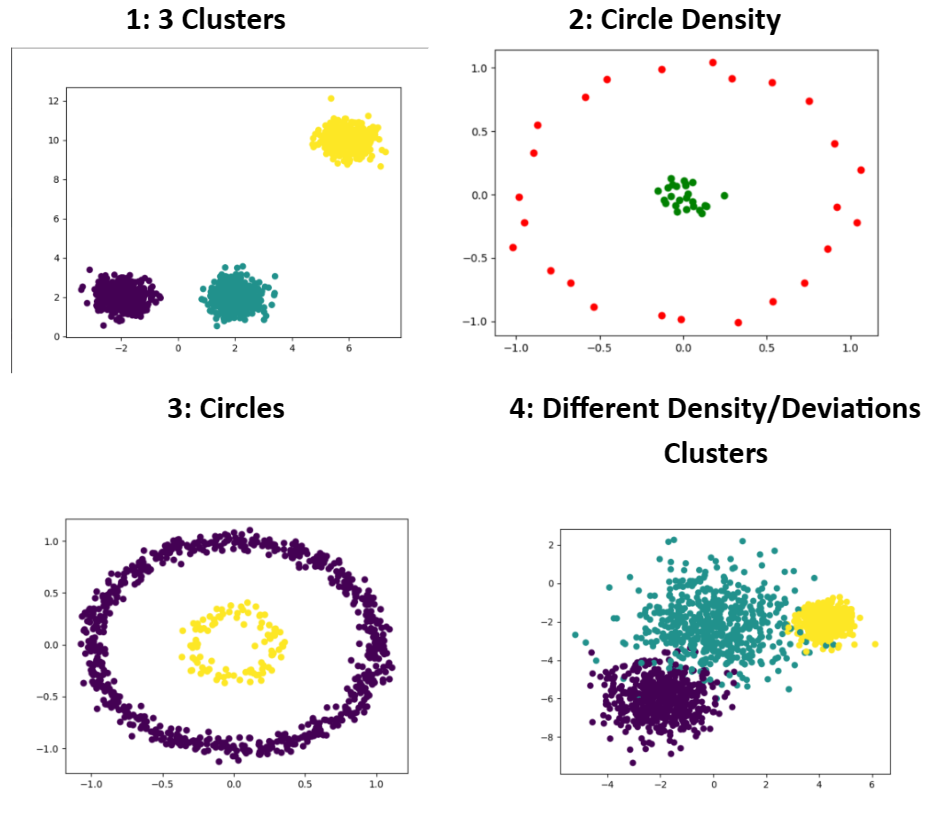
\includegraphics[width=6.8cm]{p1.png}
\end{figure}
\begin{figure}[htp]
    \centering
    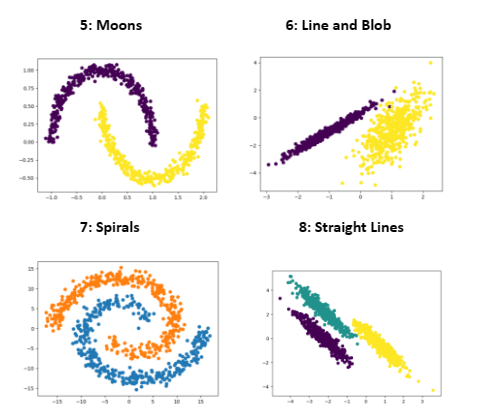
\includegraphics[width=6.8cm]{p2.png}
\end{figure}
\\\\
We chose these 8 specific datasets for a multitude of reasons. Some of them cannot be clustered well unless there is a non-linear boundary between the clusters (Spirals, Moons, Circles, Circles Density, Different Deviations Clusters). Circles Density and Different Density Clusters focuses more on the varying levels of point density between clusters. 3 Clusters is just a simple test to see if the algorithm can detect clusters linearly which was useful when designing our algorithm. Others focus on clusters that are close to each other (Line and Blob, Straight Lines, and Different Deviations Clusters). Data 7: Spirals were not created by us, but by 45deg on Github.

\section{Methods}

In total, we compared six different machine learning algorithms on the above eight datasets, all of which for descriptions are given below.

\subsection{\textbf{DBSCAN}}
DBSCAN (Density-Based Spatial Clustering of Applications with Noise) is an unsupervised clustering algorithm that groups data points into clusters based on density and proximity.  By classifying points as core, border, or noise based on local density, DBSCAN determines cluster counts and accommodates varying densities within clusters. The algorithm starts by initializing parameters, such as the radius and minimum points. It then classifies points, expands clusters from core points, assigns border points, and removes noise. DBSCAN's advantages are its flexibility, robustness to noise, and automatic cluster count determination. However, its disadvantages are its sensitivity to parameter choices and challenges with varying densities. 
\\
DBSCAN minimizes this loss function:
\begin{figure}[htp]
    \centering
    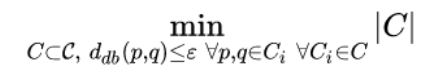
\includegraphics[width=5cm]{loss.png}
\end{figure}
\subsection{\textbf{HDBSCAN}}
HDBSCAN (Hierarchical Density-Based Spatial Clustering of Applications with Noise) is an unsupervised clustering algorithm that extends on DBSCAN. It performs DBSCAN over several different epsilon values and integrates the results. This allows HDBSCAN to perform better than DBSCAN normally, as it can detect clusters with varying densities and that would require different epsilon values if using DBSCAN.

\subsection{\textbf{K-MEANS:}}
K-means is an unsupervised machine learning algorithm where the objective is to separate a group of n observations into k groups.\\
The pseudocode for the algorithm is as follows:\\
Step 1: Choose a K, where K represents the number of centroids (i.e. clusters)\\
Step 2: Randomly select centroids positions\\
Step 3: Calculate distances between each data point and K centroids to figure out the closest cluster and assign each data point to a cluster\\
Step 4: Calculate the mean of each cluster. Use the mean value as the new centroid\\
Step 5: Repeat step 3 and 4 until any of the following condition is met:\\

 Centroids of newly formed clusters do not change

 Points remain in the same cluster

 Maximum number of iterations are reached

(Source: Yilmaz Slides 12)

\subsection{\textbf{BIRCH:}}
BIRCH (Balanced Iterative Reducing and Clustering using Hierarchies) is a hierarchical  unsupervised machine learning clustering algorithm that is tended to be used to perform over large datasets but manages to be memory and space efficient by summarizing the dataset and then running clustering on that instead. BIRCH can only be run on metric data or qualitative data. 
\\\\
It summarizes dense region information or clusters by creating Clustering Feature entries which take the following form: (Number of data points in cluster, Linear sum of all the data points, squared sum of the data points)
\\\\
BIRCH creates a Clustering Feature height-balanced tree where each leaf represents a subcluster and each entry (non-leaf) which points to its children leaves which is what it’s made up from.
\\\\
BIRCH takes two parameters: threshold (max amount of data points for an entry), branching factor (max features per entry), and the final amount of clusters returned. These control how big the tree is.
\\\\
BIRCH does the following steps to add a datapoint to a tree:

\begin{enumerate}
    \item First, recursively go down the tree and find the child node that is closest to the data point using Euclidean distance or some distance measure.
    \item Modify the leaf to add the data point either by editing a currently existing entry within or creating a new one.
    \item If there are too many features already on this leaf, split the leaf and create a new one from the same parent. If the parent has the maximum number of children we split the parent. Basically recursively split upwards if needed.
\end{enumerate}

\subsection{\textbf{WARD:}}
Ward’s method is a hierarchical bottoms-up clustering algorithm by Joe H. Ward, Jr. The main difference between it and other hierarchical algorithms is how it measures the distance between clusters. When it creates the next higher level of the clustering tree, the algorithm attempts to generate all possible clusters. While Ward initially suggested that each stage‘s merging based on "any function that reflects the investigator's purpose" (Ward, 258). He provided the following possible method. 
\\
When testing the merge between two clusters, Ward’s method calculates the possible centroid of the combined centroid and then calculates the total squared Euclidean distance from the centroid to all of the cluster’s points. The following is the equation to determine a point’s variance:
\\
\begin{figure}[htp]
    \centering
    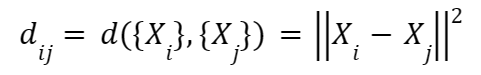
\includegraphics[width=5cm]{wad.png}
\end{figure}
\\
The two clusters that provide the smallest total squared distance are combined in the next level.

\subsection{\textbf{MODIFIED K-MEANS}}
This algorithm works by transforming the n dimension non-linearly distributed data into n+1 dimension data using cluster density as the n+1 attribute. Cluster density is most simply estimated as the distance to the nearest point to minimize calculations. The other modification is that Manhattan distance is used instead of Euclidean distance in order to amplify how important cluster density is (Manhattan distance is longer than Euclidean). Other than this, the steps of this algorithm are identical to the K-means clustering algorithm shown above.

\section{Experiments}
 In our experiments, we wanted to compare how different clustering algorithms performed against each other for nonlinearly distributed data and their application to other general datasets. We used the k-value that was the true number of classes for all algorithms because our intent was to compare the algorithms themselves, without having the process of selecting the k-value impede the process.
\\\\
The primary metrics we used for our experiments were speed, homogeneity, and completeness. Homogeneity and completeness were imported from the scikit-learn library (1.3.2). Speed was the time (measured in seconds) it took for a machine learning algorithm to run on Google Colab, which we used for consistency. Homogeneity was the measure of if a specific cluster’s data points all have the same actual classification, ranging from 0.0 to 1.0, where 1.0 represents true homogeneity. Completeness was the measure of whether or not all of the data points with the same actual classification are in a cluster together, ranging from 0.0 to 1.0, where 1.0 represents all are in the same cluster.

\section{Results}
\subsection{HDBSCAN}
\begin{figure}[htp]
    \centering
    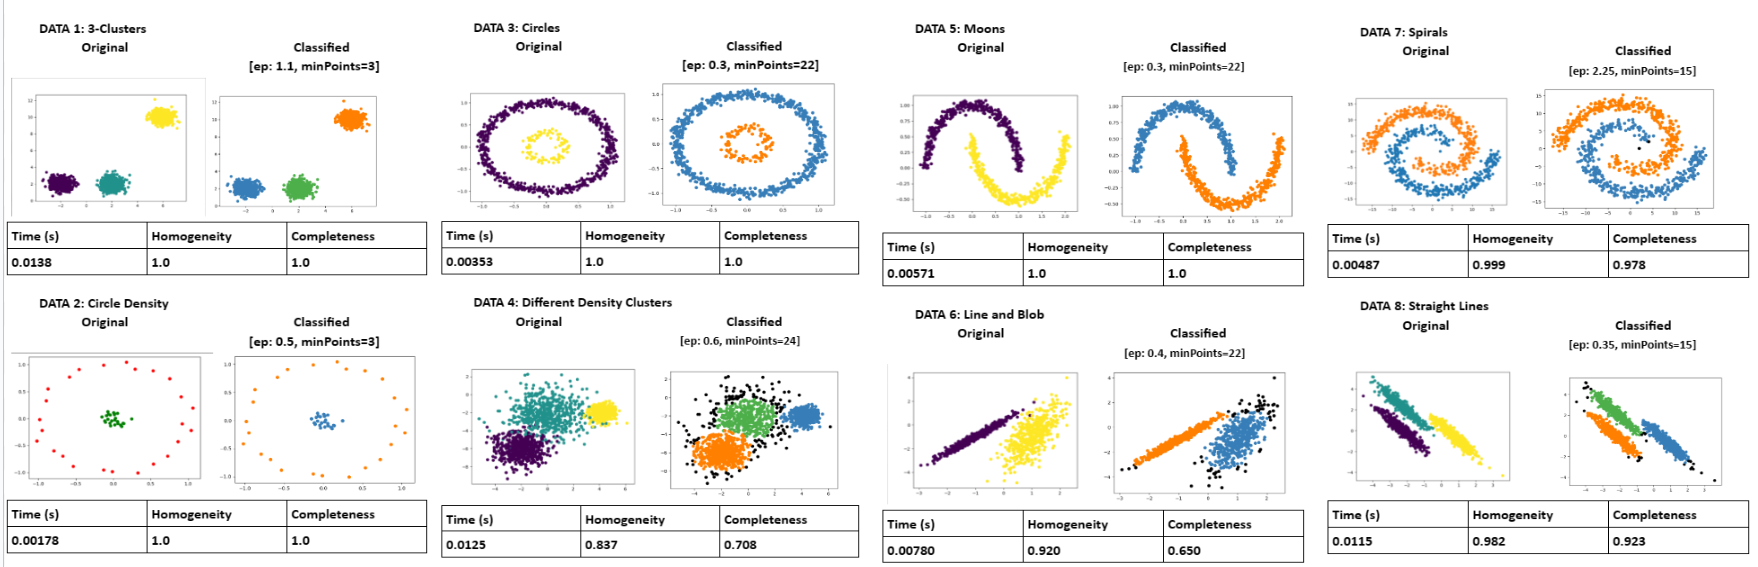
\includegraphics[width=8cm]{d1.png}
\end{figure}
\subsection{DBSCAN}
\begin{figure}[htp]
    \centering
    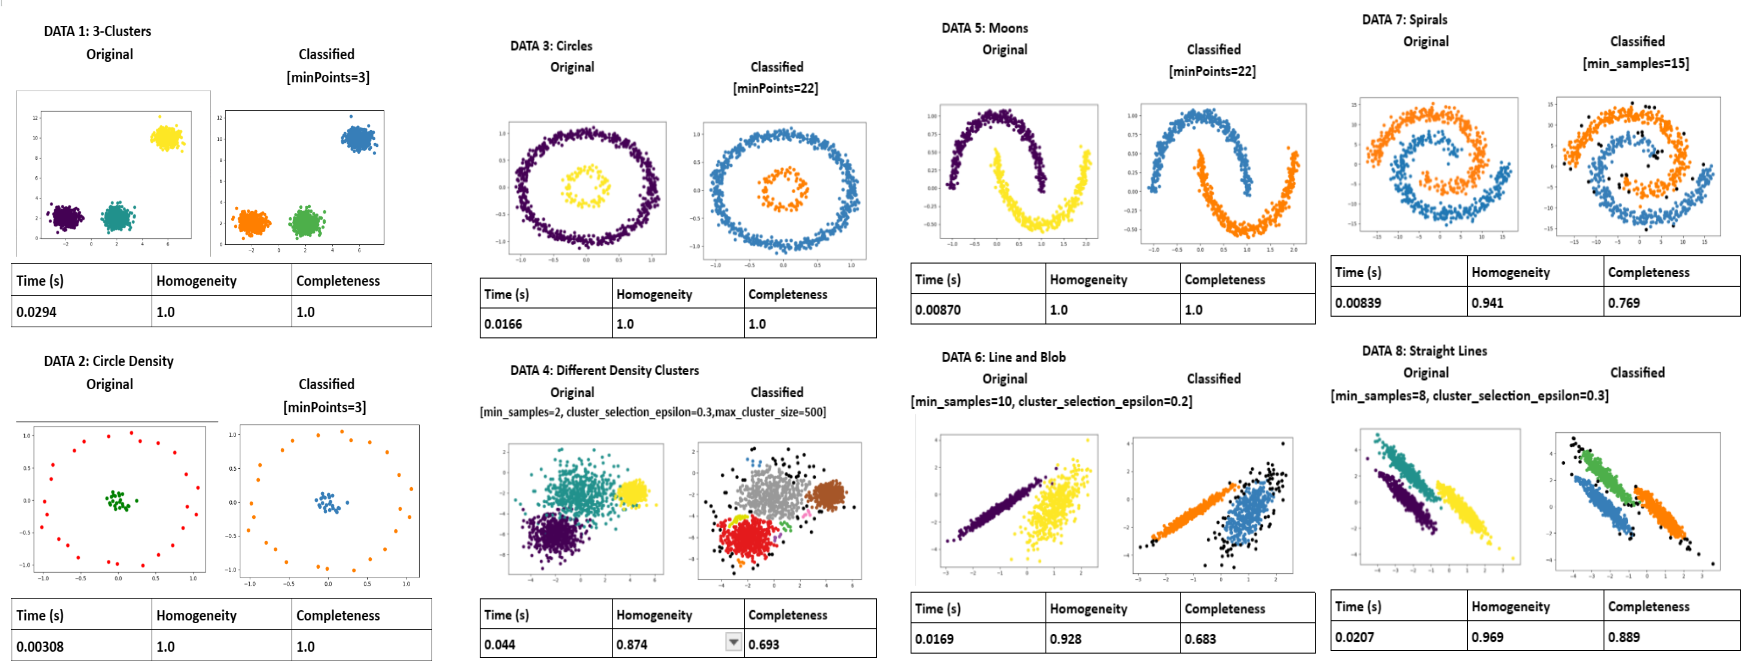
\includegraphics[width=8cm]{d2.png}
\end{figure}
\subsection{K-Means}
\hspace{1cm}
\begin{figure}[htp]
    \centering
    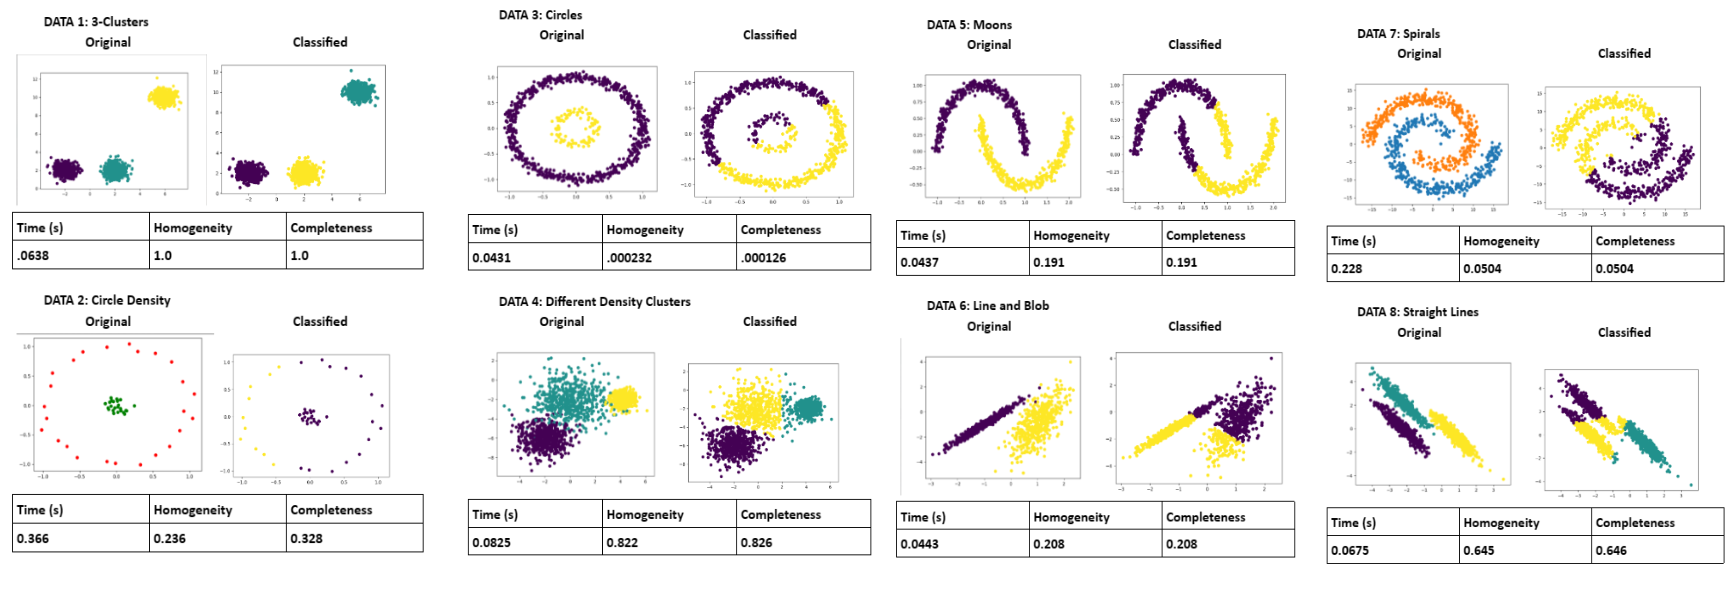
\includegraphics[width=8cm]{d3.png}
\end{figure}

\subsection{Birch}
\begin{figure}[htp]
    \centering
    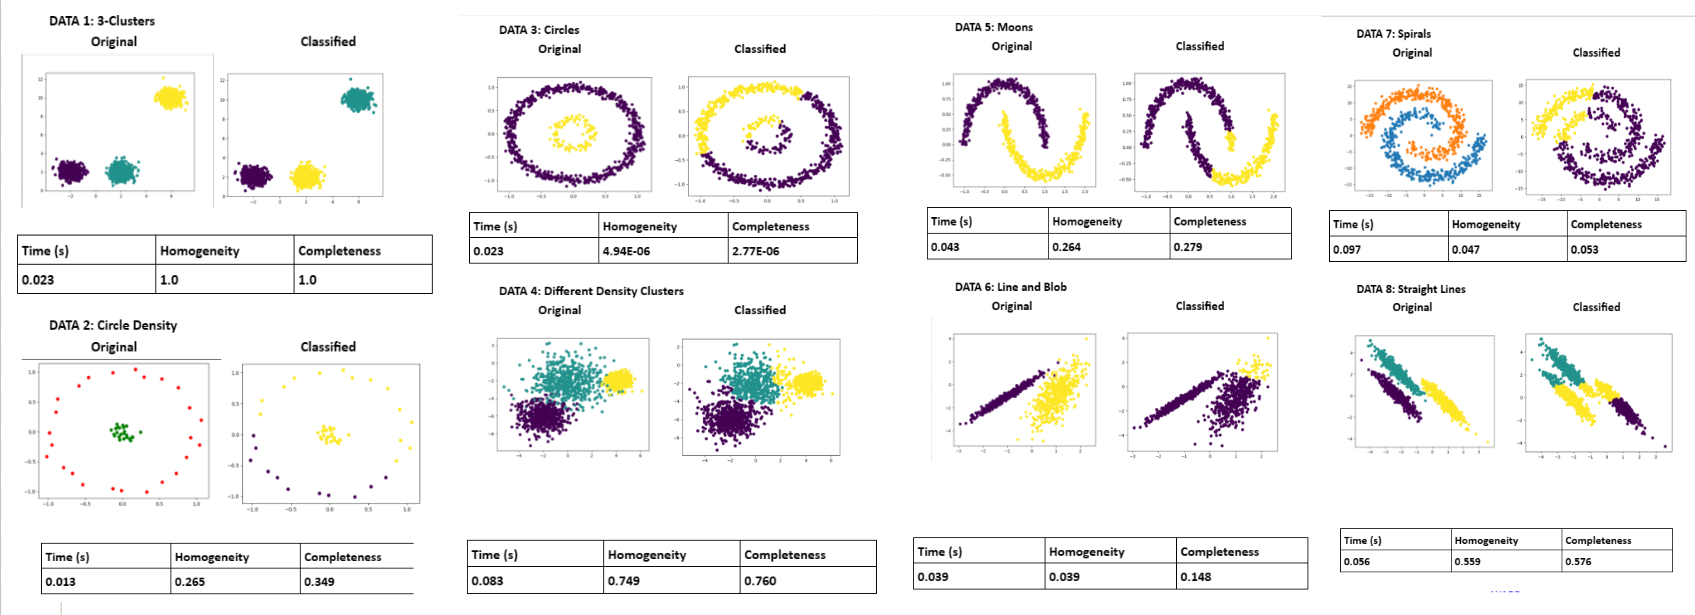
\includegraphics[width=8cm]{d4.png}
\end{figure}

\subsection{Ward}
\begin{figure}[htp]
    \centering
    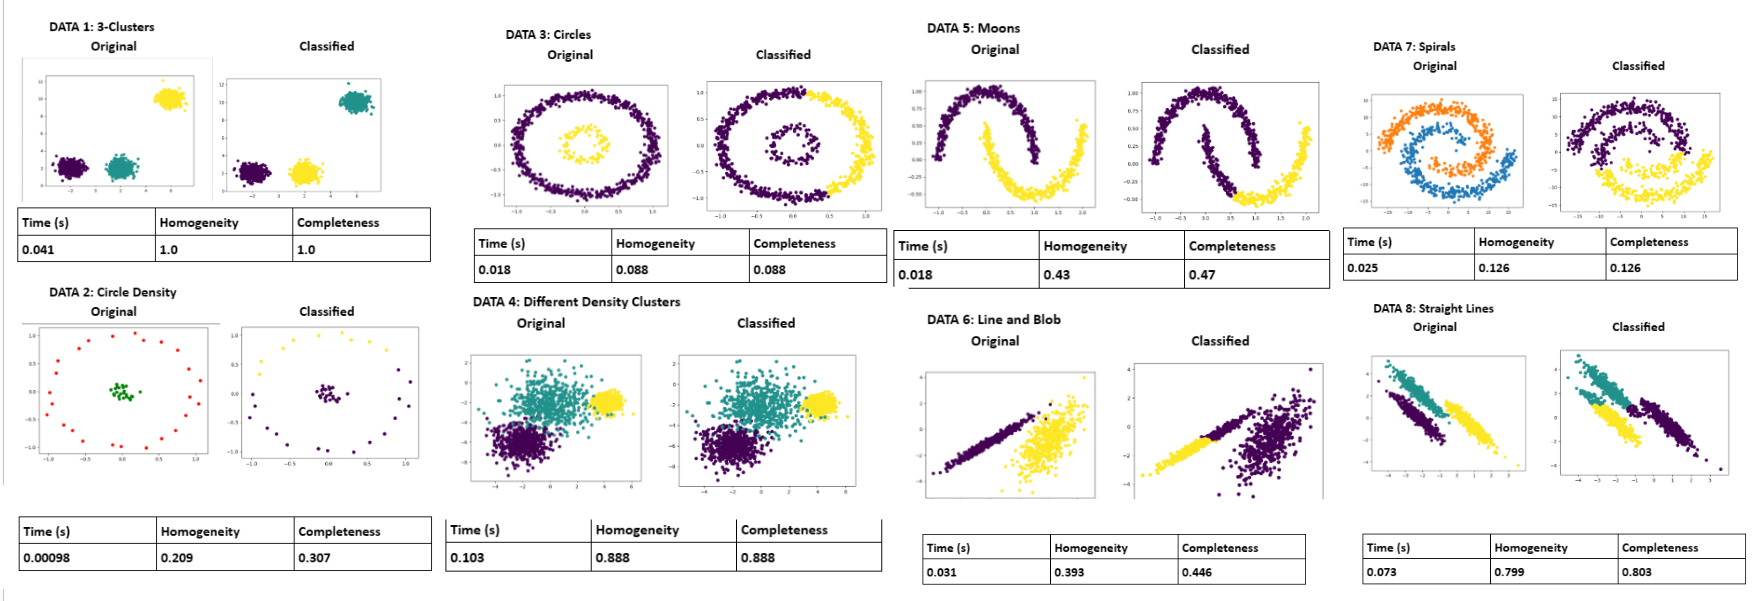
\includegraphics[width=8cm]{d5.png}
\end{figure}

\subsection{Modified K-Means}
\begin{figure}[htp]
    \centering
    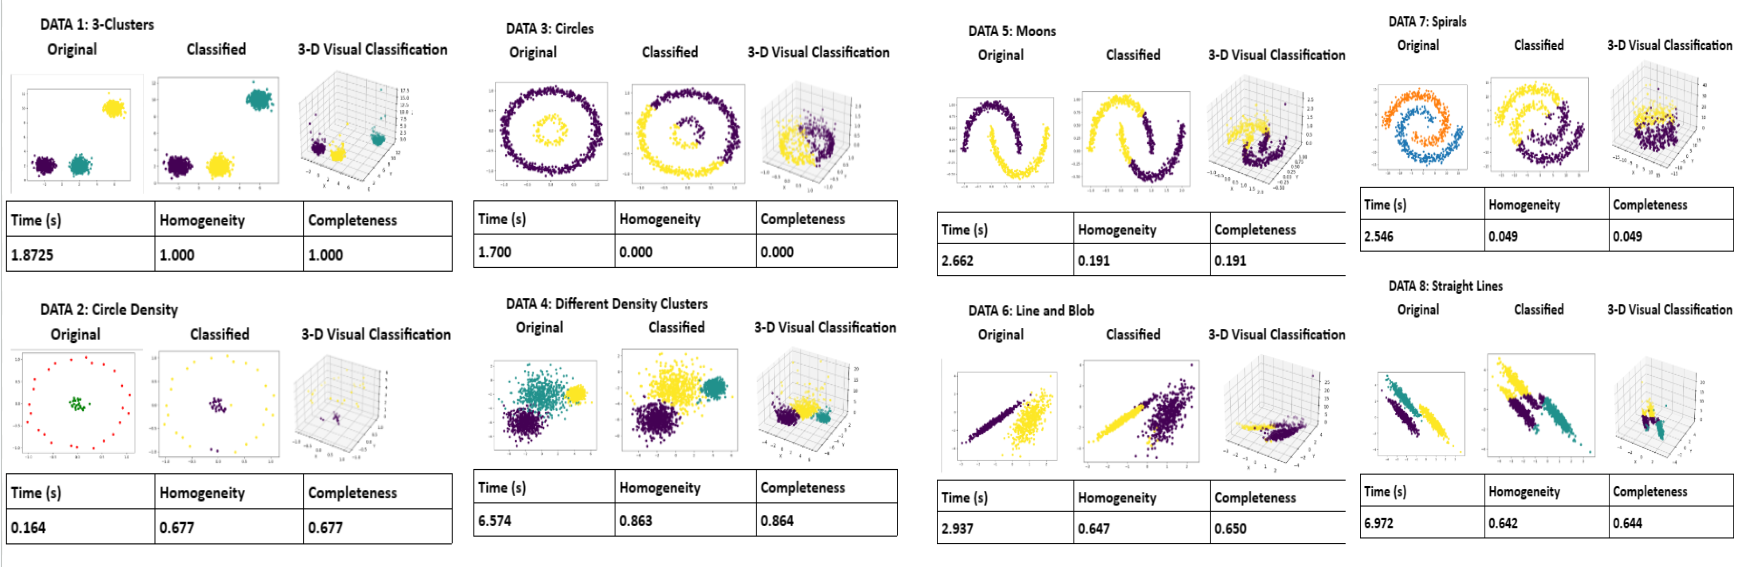
\includegraphics[width=8cm]{d6.png}
\end{figure}
\section{Discussion}
\subsection{ \textbf{SETUP DETAILS}}

As mentioned before, in our experiment we only used the 8 datasets for each of the 6 algorithms. Each of these 8 datasets had something unique about them. The majority of these datasets could only be classified using nonlinear boundaries, while others reflected on close clusters or different densities. Since we were using unsupervised classification algorithms and because all of these algorithms were easy to deploy, there was no need for any training and therefore there was no overfitting. In order to get a better understanding of which algorithm is better, algorithms that required a k-value parameter were given the true k-value of that dataset. Parameters are chosen in testing by slowly adjusting values until we reach the best possible performance values. We used the sci-kit learn library implementations of all algorithms besides modified k-Means and k-Means. We used numpy and matplotlib for plotting out results and visuals.
\textbf{
\subsection{PERFORMANCE METRICS USED}
}
\textbf{Homogeneity} [0.0-1.0] - The measure of how pure the algorithm’s clusters are using true classifications. For example, if one of our algorithms created a cluster with only two points but these two points actually have entirely different classification, we would have the worst homogeneity of 0.0 (because the cluster is 50/50 split in reality). Equations below:
\\
\begin{figure}[htp]
    \centering
    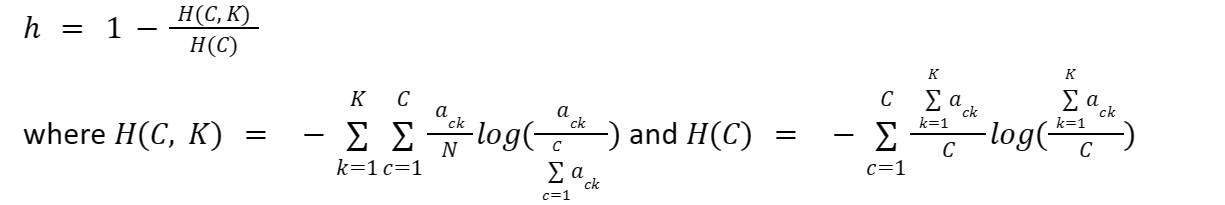
\includegraphics[width=9.5cm]{gomo.png}
\end{figure}
\\
and N is the number of data points, C is the number of class labels, K is the amount of clusters and $a_{ck}$ is the amount of data points belonging to cluster K and has class c.\\
\\
\textbf{Completeness} [0.0-1.0] - The measure of how many data points belonging to a specific classification are in the exact same cluster. For example, if the original dataset contained 50 data points classified with the label “Fire” and our algorithm classified all of those 50 data points with the label “Fire”, we have 1.0 completeness. Equations below: 
\\
\begin{figure}[htp]
    \centering
    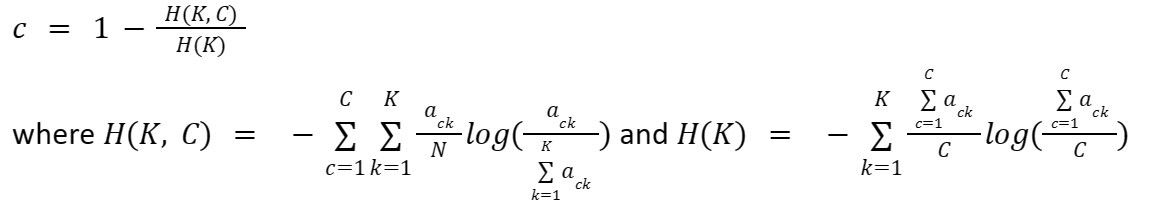
\includegraphics[width=9cm]{comp.png}
\end{figure}
\\
and N is the number of data points, C is the number of class labels, K is the amount of clusters and $a_{ck}$ is the amount of data points belonging to cluster K and has class c.\\
\\
\textbf{Elapsed time} [Seconds]- Time it took for the algorithm to completely classify the dataset
\\
\\We did not use general accuracy (what percentage of points were classified correctly) because of how usually unsupervised classification algorithms (at least sci-kit learn implementations) tend to assign attributes arbitrarily, meaning while usually the algorithm finds the correct groupings, it’ll slap a random classification on it. Therefore, we couldn’t provide ROC curves or confusion matrices.
\textbf{
\subsection{HDBSCAN and DBSCAN}
}
These two algorithms had the most accurate cluster classifications except on the following datasets: Different Density/Deviation Clusters; Straight Lines; and Line and Blob. This is expected though because DBSCAN and HDBSCAN rely on the idea of core-points and epsilon values to connect core points and non-core points in order to grow clusters and in those datasets, while there are often times centralized clusters, the clusters slowly spread out at its edges making them more sparser there, creating a less even non-uniform density within the cluster, which makes finding a good epsilon value quite difficult. While HDBSCAN is an improvement to DBSCAN, it is an improvement based on the measure of classifying more clusters with different densities compared to each other. This is why in Dataset 4, HDBSCAN finds many possible clusters and takes a loss to its completeness.
\textbf{
\subsection{BIRCH AND WARD}
}
BIRCH and Ward had nearly identical results. They were successful mainly on the 3-cluster and different density cluster datasets; they had very partial success on the straight lines and line and blob dataset, while almost completely misclassifying the remaining four datasets. While Ward’s method is good at minimizing variance within a cluster, not every dataset’s actual cluster adheres to this principle. BIRCH’s main positive being memory and space efficiency on bigger numbers of multi-dimensional data is not shown here and thus doesn’t rank high. 
\subsection{\textbf{MODIFIED K-MEANS/K-MEANS}}
While our modified kMeans algorithm was still unable to perform well on datasets where clusters are bounded by non-linear lines because it is an extension on kMeans, it still had an improvement in the following datasets: Circle Density, Different Density/Deviation Clusters, Line and Blob. Our new algorithm helps significantly on clear clusters where there is a differing uniform density but still faces some issues where same density and deviation clusters are close to each other. For example, Dataset 4 faces this issue where some points on the outer region of clusters will be assigned to the same z-level as other clusters because the clusters are very close to each other and will then have the same calculated nearby-point distance. This makes it easy for points to get assigned to a different cluster and clusters with higher deviation to decrease in size. Our new algorithm also is much slower because we’ve added an additional axis to each point.

 \section{Conclusion}
In conclusion, the DBScan and HDBScan algorithms had the greatest success on our non-linearly distributed datasets. The modified K-means algorithm performed somewhere in the middle, while Birch, Ward, and regular K-means performed the most poorly. Overall, our work creating a new algorithm seems to be at least a partial success, as our modified K-means algorithm performed extremely well on differentiating blobs of differing densities. On the other hand, our modified K-means algorithm still struggled with differentiating between nonlinear clusters which had similar densities.
\\\\
We’ve also learned limitations on HDBScan and DBScan regarding their inability to work with datasets where clusters have big standard deviations and learned new clustering algorithms like BIRCH and Ward’s method which tackle other clustering problems.
\section{Future Work}

Given more time for this project, we would likely consider using different distance functions other than Manhattan (Taxicab) distance. We would also consider the use of the K-means modified algorithm beyond 2D linearly distributed data, as most data in the real world has a high number of dimensions. More time would also allow us to find the most optimal values for each algorithm’s parameters. Finally, we could also just amplify the importance of cluster density by multiplying the z-values by a constant, to reduce the effect of close clusters.

\section{Contributions}

Sol was responsible for creating the modified K-means algorithm of changing the dimension n to n+1, and writing the abstract and introduction. Tao was responsible for creating/providing the datasets, regulating what performance metrics to use, testing Ward’s method, BIRCH, DBScan, and HDBScan, writing sections on BIRCH and Ward’s method as well. Aadhitya was responsible for regular K-means data collection.

 



 



% WARNING
%-------------------------------------------------------------------
% Please note that we have included the references to the file aa.dem in
% order to compile it, but we ask you to:
%
% - use BibTeX with the regular commands:
%   \bibliographystyle{aa} % style aa.bst
%   \bibliography{Yourfile} % your references Yourfile.bib
%
% - join the .bib files when you upload your source files
%-------------------------------------------------------------------

\begin{thebibliography}{}
  \bibitem[1]{awdjiaw} 45deg (2018) Generating Spiral Dataset for Classifying in Python. Github https://gist.github.com/45deg/e731d9e7f478de134def5668324c44c5
  
  \bibitem[Baker(1966)]{baker} Campello, Ricardo JGB, Davoud Moulavi, and Joerg Sander. 2013. “Density-Based Clustering Based on Hierarchical Density Estimates.” In Pacific-Asia Conference on Knowledge Discovery and Data Mining, 160–72. Springer.

   \bibitem[Balluch(1988)]{balluch} D. Deng, "DBSCAN Clustering Algorithm Based on Density," 2020 7th International Forum on Electrical Engineering and Automation (IFEEA), Hefei, China, 2020, pp. 949-953

   \bibitem[4]{awdaw} Harris, C.R., Millman, K.J., van der Walt, S.J. et al. Array programming with NumPy. Nature 585, 357–362 (2020). DOI: 10.1038/s41586-020-2649-2. (Publisher link).

   \bibitem[Hi(2000)]{awdnaow} J. D. Hunter, "Matplotlib: A 2D Graphics Environment", Computing in Science & Engineering, vol. 9, no. 3, pp. 90-95, 2007. DOI: https://doi.org/10.5281/zenodo.10150955
   
   \bibitem[Cox(1980)]{cox} Karayiannis, Nicolaos B. and Randolph-Gips, Mary M. ‘Non-Euclidean C-means Clustering Algorithms’. 1 Jan. 2003 : 405 – 425.

   \bibitem[Cox(1969)]{cox69} Martin Ester, Hans-Peter Kriegel, Jörg Sander, and Xiaowei Xu. 1996. A density-based algorithm for discovering clusters in large spatial databases with noise. In Proceedings of the Second International Conference on Knowledge Discovery and Data Mining (KDD'96). AAAI Press, 226–231.

   \bibitem[8]{awd} Scikit-learn: Machine Learning in Python, Pedregosa et al., JMLR 12, pp. 2825-2830, 2011.
   
   \bibitem[Mizuno(1980)]{mizuno} Scitovski, R., Sabo, K. DBSCAN-like clustering method for various data densities. Pattern Anal Applic 23, 541–554
   
   \bibitem[Tscharnuter(1987)]{tscharnuter} Ward, J. H., Jr. (1963), "Hierarchical Grouping to Optimize an Objective Function", Journal of the American Statistical Association, pp. 236–244.
  
   \bibitem[Terlevich(1992)]{terlevich} Zhang, T.; Ramakrishnan, R.; Livny, M. (1996). "BIRCH: an efficient data clustering method for very large databases". Proceedings of the 1996 ACM SIGMOD international conference on Management of data - SIGMOD '96. pp. 103–114.

\end{thebibliography}

\end{document}
%
%%%%%%%%%%%%%%%%%%%%%%%%%%%%%%%%%%%%%%%%%%%%%%%%%%%%%%%%%%%%%%
Example below of non-structurated natbib references  
To use the v8.3 macros with this form of composition of bibliography, 
the option "bibyear" should be added to the command line 
"\documentclass[bibyear]{aa}".
%%%%%%%%%%%%%%%%%%%%%%%%%%%%%%%%%%%%%%%%%%%%%%%%%%%%%%%%%%%%%%


%
%%%%%%%%%%%%%%%%%%%%%%%%%%%%%%%%%%%%%%%%%%%%%%%%%%%%%%%%%%%%%%
Examples for figures using graphicx
A guide "Using Imported Graphics in LaTeX2e"  (Keith Reckdahl)
is available on a lot of LaTeX public servers or ctan mirrors.
The file is : epslatex.pdf 
%%%%%%%%%%%%%%%%%%%%%%%%%%%%%%%%%%%%%%%%%%%%%%%%%%%%%%%%%%%%%%

%
%-------------------------------------------------------------
%               Appendices have to be placed at the end, after
%                                        \end{thebibliography}
%-------------------------------------------------------------
\end{thebibliography}



%
%
\end{document}

%
%-------------------------------------------------------------
%          For the appendices, table longer than a single page
%-------------------------------------------------------------

% Table will be print automatically at the end of the document, 
% after the whole appendices

\begin{appendix} %First appendix


% In the appendices do not forget to put the counter of the table 
% as an option

\longtab[1]{
\begin{longtable}{lrcrrrrrrrrl}
\caption{Line data and abundances ...}\\
\hline
\hline
Def & mol & Ion & $\lambda$ & $\chi$ & $\log gf$ & N & e &  rad & $\delta$ & $\delta$ 
red & References \\
\hline
\endfirsthead
\caption{Continued.} \\
\hline
Def & mol & Ion & $\lambda$ & $\chi$ & $\log gf$ & B & C &  rad & $\delta$ & $\delta$ 
red & References \\
\hline
\endhead
\hline
\endfoot
\hline
\endlastfoot
A & CH & 1 &3638 & 0.002 & $-$2.551 &  &  &  & $-$150 & 150 &  Jorgensen et al. (1996) \\                    
\end{longtable}
}% End longtab
\end{appendix}

%-------------------------------------------------------------
%                   For appendices and landscape, large table:
%                    in the preamble, use: \usepackage{lscape}
%-------------------------------------------------------------

\begin{appendix} %First appendix
%
\longtab[1]{
\begin{landscape}
\begin{longtable}{lrcrrrrrrrrl}
...
\end{longtable}
\end{landscape}
}% End longtab
\end{appendix}

%%%% End of aa.dem
